\documentclass[a4paper,11pt]{book}
\usepackage{import}
\usepackage{preamb}

\makeindex

\begin{document}

\small
\begin{multicols}{3}

%\maketitle

\thispagestyle{empty}
\scriptsize
\newpage


\begin{subbox}{subbox}{}
\centering
\Large{\textbf{Network Science   \\ Cheatsheet}}
\end{subbox}

\begin{multibox}{2}
\begin{subbox}{subbox}{}
\centering

\includegraphics[width=0.8\textwidth]{pics/logo.png}
\end{subbox}
\begin{subbox}{subbox}{}
\centering
Made by \\
\large{
Remy Cazabet
}
\end{subbox}
\end{multibox}
% \section{Blocks and Community structure}


\begin{subbox}{subbox}{}
\centering
\Large{\textbf{Dynamic Networks}}
\end{subbox}


\begin{subbox}{subbox}{Disclaimer}
Dynamic network analysis as introduced here is a recent and still not fully mature field, with a large number of contributions, for which we cannot know yet which one will stand the test of time. This is therefore \textit{my} vision of the dynamic network field  \textit{as of today}.
\end{subbox}



\begin{textbox}{Ubiquity of Dynamic Networks}

Most real networks are in fact dynamic: nodes and edges appear and disappear with time. Think of friendship in social networks, flight routes or any human interactions. Networks are often analyzed as static objects because 1)it's harder to obtain dynamic information, 2)Taking dynamic into account makes some analysis more difficult. 

While more and more aspects of our life become linked to digital technology, datasets with fine temporal information also become more and more common.
\end{textbox}




\begin{textbox}{Snapshots \& Aggregated Networks}

Dynamic networks can sometimes be represented as sequences of static graphs.
These graphs can be obtained by two processes:
\begin{itemize}
    \item \textbf{Snapshots} correspond to the state of a network at a particular point in time, e.g., all follower/followees relationship at a particular second
    \item \textbf{Aggregated Networks} are obtained by cumulating information over a period of time, e.g., in a phone call network, in the snapshot representing year 2020, an edge exists between two individuals if they called each other at least once over the year 2020.
\end{itemize}
\end{textbox}

\begin{textbox}{Interactions or Relation?}
Dynamic networks can be used to represent different types of real data. In particular, they can be used to represent networks of \textbf{relations} and networks of \textbf{interactions}. For instance, friendships, acquaintances, physical wires, roads, etc. can be thought as \textit{relations}, while e-mails, phone calls, instant messages, physical contacts, etc. are \textit{interactions}.

There is often a relation between these two notions: interactions tend to occur between entities having a relation, and/or relations tend to form between entities having interactions.
\end{textbox}

\begin{textbox}{Dynamic Network Properties}
Independently of the studied data, dynamic networks can have various properties:
\begin{itemize}
    \item \textbf{Edge} presence can be \textbf{punctual} or \textbf{with duration}
    \item \textbf{Node} presence can be \textbf{unspecified}, \textbf{punctual} or \textbf{continuous}
    \item If \textbf{time is continuous}, it can be \textbf{bounded} on a period of analysis or \textbf{unbounded}
    \item If \textbf{nodes} have attributes, they can be \textbf{constant} or \textbf{time-dependent}
    \item If \textbf{edges} have weights, they can be \textbf{constant} or \textbf{time-dependent}
\end{itemize}
\end{textbox}






\begin{textbox}{Vocabulary}
Many different names have been used for networks changing with time, but there is no broad consensus in the literature on the meaning of those terms, unless they are used with an explicit reference to a paper defining them. Here is a list of the most popular:
\begin{itemize}
    \item \textbf{Dynamic Networks} and \textbf{Dynamic Graphs}
    \item \textbf{Longitudinal Networks}
    \item \textbf{Evolving Graphs}
    \item \textbf{Link Streams} \& \textbf{Stream Graphs} (\cite{latapy2018stream})
    \item \textbf{Temporal Networks}, \textbf{Contact Sequences} and \textbf{Interval Graphs} (\cite{holme2012temporal})
    \item \textbf{Time Varying Graphs} (\cite{casteigts2012time})
\end{itemize}
\end{textbox}


% \begin{textbox}{From data to network representation}
% To see how the same data can give birth to different dynamic network representation, let's take a simple example: the SocioPatterns projet \footcite{barrat2013empirical} has collected several physical interaction datasets between individuals in various contexts, such as schools or hospitals. Wearable sensors collect every face-to-face interaction at a high frequency between a group of subjects over an extended period of time. For practical reasons, data collection is made for the whole setting every 20 seconds, in a synchronous fashion. The publicly provided data therefore consists in a file containing all those captured interactions, as triplets $<T,U1,U2>$, with $T$ the timestamp of the interaction, $U1$ and $U2$ the face-to-face individuals. There are therefore several ways to interpret such data:
% \begin{itemize}
%     \item \textbf{Snapshots}: Each 20s, a snapshot of all on-going conversations is captured. Each of these snapshots could be studied as a conventional static graph. (Nodes and edges presence time are punctual)
%     \item \textbf{Link Stream}: Each triplet is a link of the link stream, it corresponds to an observed interaction between individuals. (Nodes presence time is not specified, edge presence time is punctual)
%     \item \textbf{Interval Graphs}: Individuals do not interact punctually but over periods of time, usually longer than 20s. Technical reasons force to capture the state of these persistent interactions periodically every 20s. To model more accurately the observed phenomenon, one should create continuous intervals for each pair of node interacting repeatedly every 20s over a period, lasting from the first to the last observation of the series. (Nodes and edge presences are continuous with duration)
% \end{itemize}
% \end{textbox}




\begin{textbox}{Slowly Evolving/Degenerate}
Beyond the nature of the data and the chosen representation, a critical difference defining how a dynamic network can be analyzed is whether it is a \textbf{Slowly Evolving Network (SEN)} or \textbf{Degenerate}. In a SEN network, to each instant corresponds a well defined graph, that can be studied with usual tools of network science. In a degenerate temporal network, a meaningful graph can be obtained only when aggregating it over a period $\Delta$.
\end{textbox}




\begin{textbox}{Analyzing SEN}
A slowly evolving network can easily be studied by the tools already defined on static graphs. For any instant (discrete or continuous), one can compute network descriptors (density, clustering coefficient, etc.), node descriptors (centralities), reachability, etc.
\end{textbox}


\begin{textbox}{Analyzing degenerate networks}
A degenerate network can always be transformed into a SEN by aggregating it using time windows, fixed (yielding snapshots, i.e., discrete SEN) or sliding (yielding continuous SEN). But a more powerful solution is to study them in their original form, without loosing any temporal information through aggregation. This however requires new definitions. 
\end{textbox}


\begin{textbox}{Stream Graph (SG)- Definition}
Stream Graphs have been proposed in \footcite{latapy2018stream} as a generic formalism --it can represent any type of dynamic networks, continuous, discrete, with or without duration, with the objective or redefining typical notions of graphs on dynamic networks, including degenerate ones.

Let's define a Stream Graph 
\[S=(T,V,W,E)\]


\begin{tabular}{p{0.08\textwidth}|p{0.8\textwidth}}\scriptsize

$T$ & \textbf{Set of Possible times} (Discrete or Time intervals) \\

$V$ & \textbf{Set of Nodes} \\

$W$ & \textbf{Vertices presence time} $V \times T$ \\
$E$ & \textbf{Edges presence time} $V \times V \times T$ \\


\end{tabular}
\end{textbox}



\begin{textbox}{SG - Time-Entity designation}
It is useful to work with Stream Graphs to introduce some new notions mixing entities (nodes, edges) and time:


\begin{tabular}{p{0.08\textwidth}|p{0.8\textwidth}}\scriptsize
$V_{t}$ & \textbf{Nodes At Time}: set of nodes present at time $t$\\
$E_{t}$ & \textbf{Edges At Time}: set of edges present at time $t$\\
$G_t$ & \textbf{Snapshot}: Graph at time $t$, $G_t=(V_t,E_t)$\\
$v_t$ & \textbf{Node-time}: $v_t$ exists if node $v$ is present at time $t$\\
$(u,v)_t$ & \textbf{Edge-time}: $(u,v)_t$ exists if edge $(u,v)$ is present at time $t$ \\
$T_u$ & \textbf{Times Of Node}: the set of times during which $u$ is present\\
$T_{uv}$ & \textbf{Times Of Edge}: the set of times during which edge $(u,v)$ is present\\

\end{tabular}
\end{textbox}





\begin{textbox}{SG - Node/Edge presence}
Nodes and Edges are typically present in the graph only for a fraction of its total duration, Node/Edge presence is computed as the fraction of the total times during which it is present. Note that if time is continuous and edges are discrete, we take by convention $|T|=1$, i.e., we simply count nodes/edges presence time.


\begin{tabular}{p{0.08\textwidth}|p{0.8\textwidth}}\scriptsize

$N_u$ & \textbf{Node presence}: The fraction of the total time during which $u$ is present in the network $\frac{|T_u|}{|T|}$ \\
$L_{uv}$ & \textbf{Edge presence}: The fraction of the total time during which $(u,v)$ is present in the network $\frac{|T_{uv}|}{|T|}$ \\

\end{tabular}
\end{textbox}





\begin{textbox}{SG - Redefining Graph notions}
The general idea of redefining static network properties on Stream Graphs is that if the network stays unchanged along time, then properties computed on the stream graph should yield the same values as the same properties computed on the aggregated graph.
\end{textbox}


\begin{textbox}{SG - $N$}
The number/quantity of nodes in a stream graph is defined as the total presence time of nodes divided by the dataset duration. In general, it isn't an integer.

More formally:

\[
N=\sum_{v\in V} N_v = \frac{|W|}{|T|}
\]
For instance, $N=2$ if there are 4 nodes present half the time, or two nodes present all the time.
\end{textbox}



\begin{textbox}{SG - $L$}
The number of edges is defined as the total presence of edges divided by the total dataset duration.

More formally:

\[
L=\sum_{(u,v),u,v \in V} L_{uv}=\frac{|E|}{|T|}
\]

For instance, $L=2$ if there are 4 edges present half the time, or two edges present all the time.
\end{textbox}




\begin{textbox}{SG - Edge domain - $L_{\max}$}
In Stream Graphs, several possible definitions of ${L_{\max}}$ could exist:
\begin{itemize}
    \item Ignoring nodes duration: ${L_{\max}^1}=|V|^2$
    \item Ignoring nodes co-presence ${L_{\max}^2}=N^2$
    \item Taking nodes co-presence into account:  \\ ${L_{\max}^3}=\sum_{(u,v),u,v \in V}|T_u \bigcap T_v|$
\end{itemize}

\end{textbox}


\begin{textbox}{SG - Density - $d$}
The density in static networks can be understood as the fraction of existing edges among all possible edges,
\[
d=\frac{L}{L_{\max}}. 
\]
The definition can naturally be extended by using the definitions of $L$ and $L_{\max}$ introduced on Stream Graph. In (\cite{latapy2018stream}), the authors use ${L_{\max}^3}$. This definition can also be understood as the probability, if we take a time at random, and two nodes alive a that time at random, for them to be connected.

Note that a common way to define the density in static networks is $d=N^2$, because $N^2$ is the only way to define $L_{\max}$ in static networks, unlike in Stream Graphs. 

\centering
\vspace{0.3cm}


%\colorbox{white}{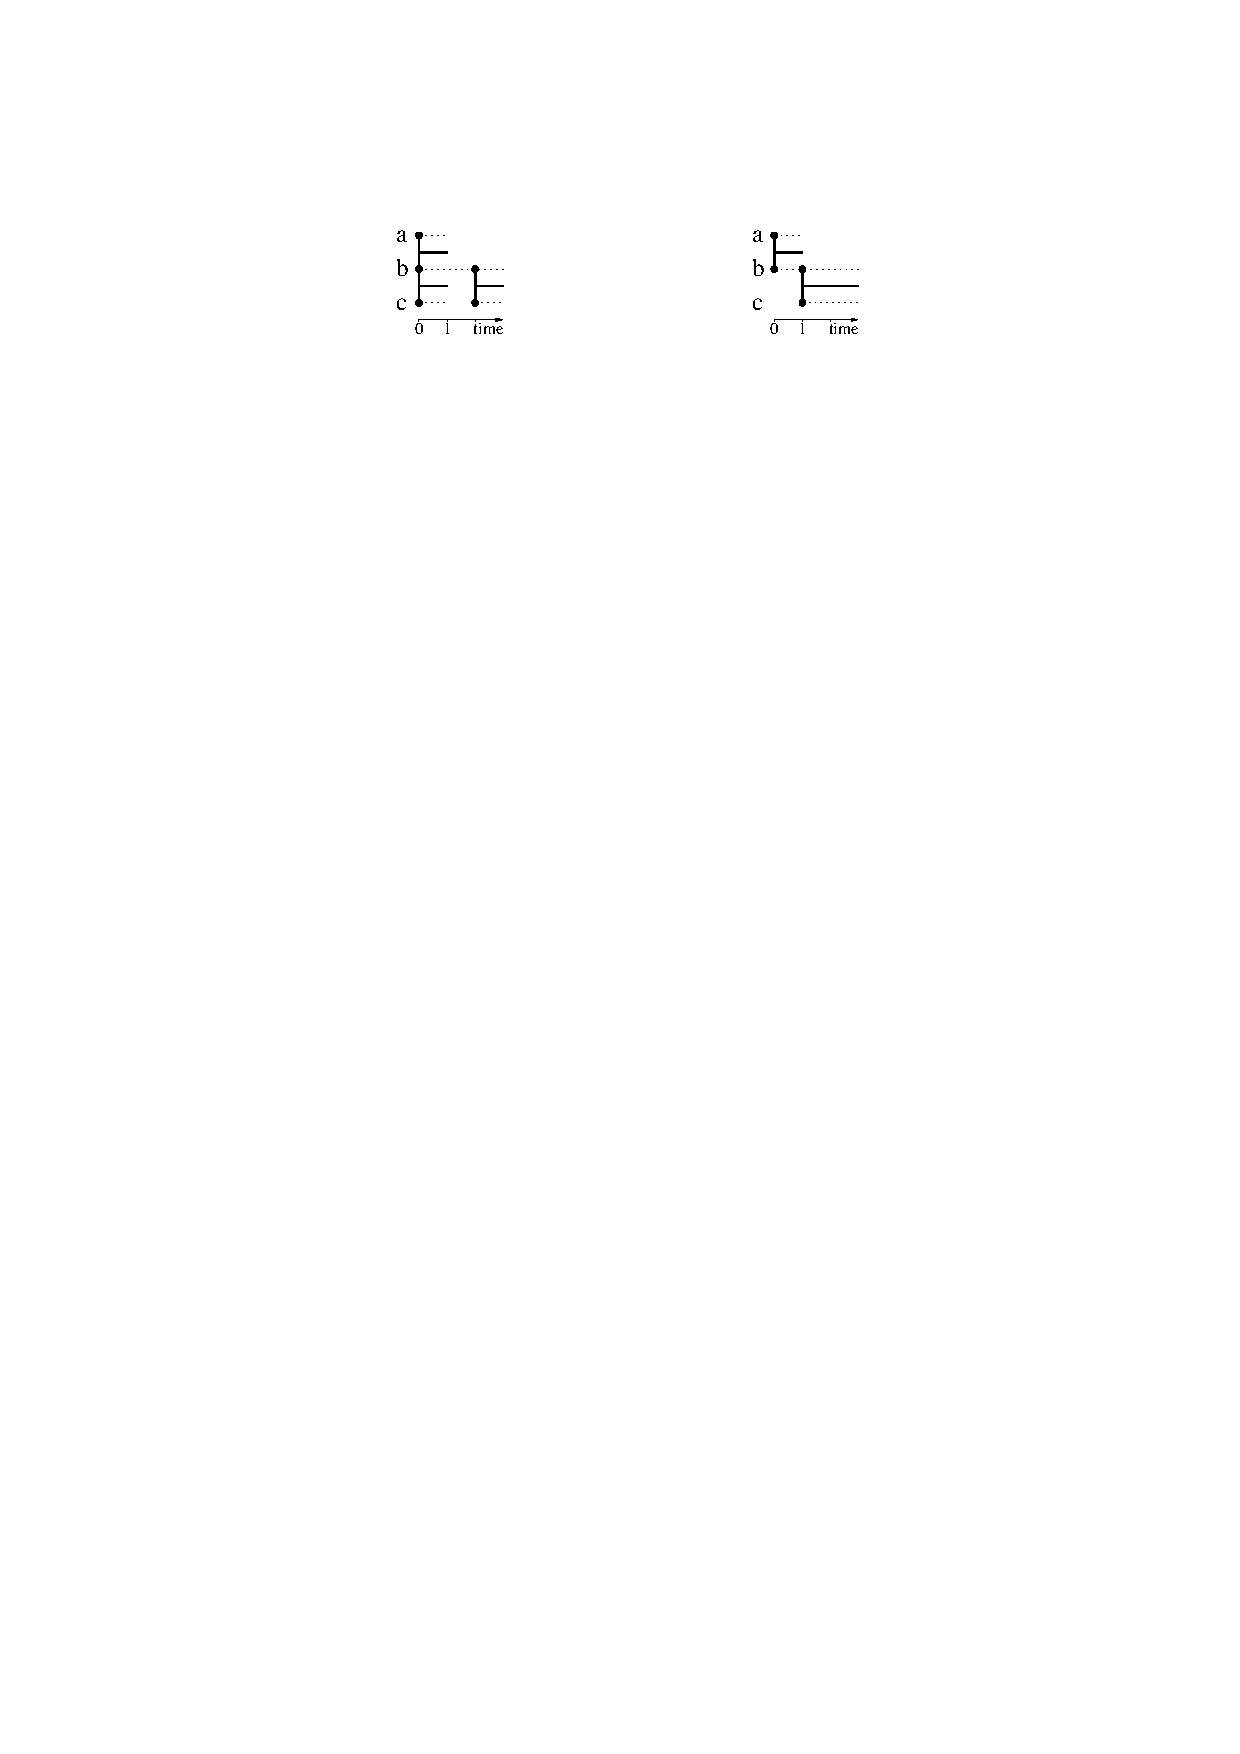
\includegraphics[width=0.9\linewidth]{pics/SGdensity.pdf}}
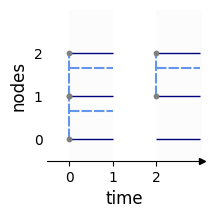
\includegraphics[width=0.3\linewidth]{pics/dynamic/d1.png}
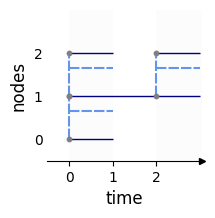
\includegraphics[width=0.3\linewidth]{pics/dynamic/d2.png}
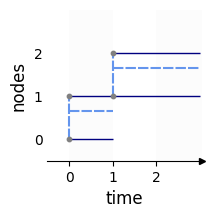
\includegraphics[width=0.3\linewidth]{pics/dynamic/d3.png}

Examples of graphs with $N=2$ nodes, $L=1$ link, but with different densities, respectively $\frac{1}{2}$ (left), $\frac{3}{4}$ (center) and 1 (right).


\end{textbox}







\begin{textbox}{SG - Clusters \& Substreams}
In static networks, a cluster is a set of nodes, and we have defined an (induced) subgraph of this cluster as a graph composed of the nodes of the cluster and the edges existing between those nodes.

In Stream Graphs, a clusters $C$ is as subset of $W$, and the corresponding (induced) substream $S(C)=(T,V,C,E(C))$, with $E(C)=\{(t,(u,v)) \in E, (t,u),(t,v) \in C\}$.

\centering

\vspace{0.3cm}

%\colorbox{white}{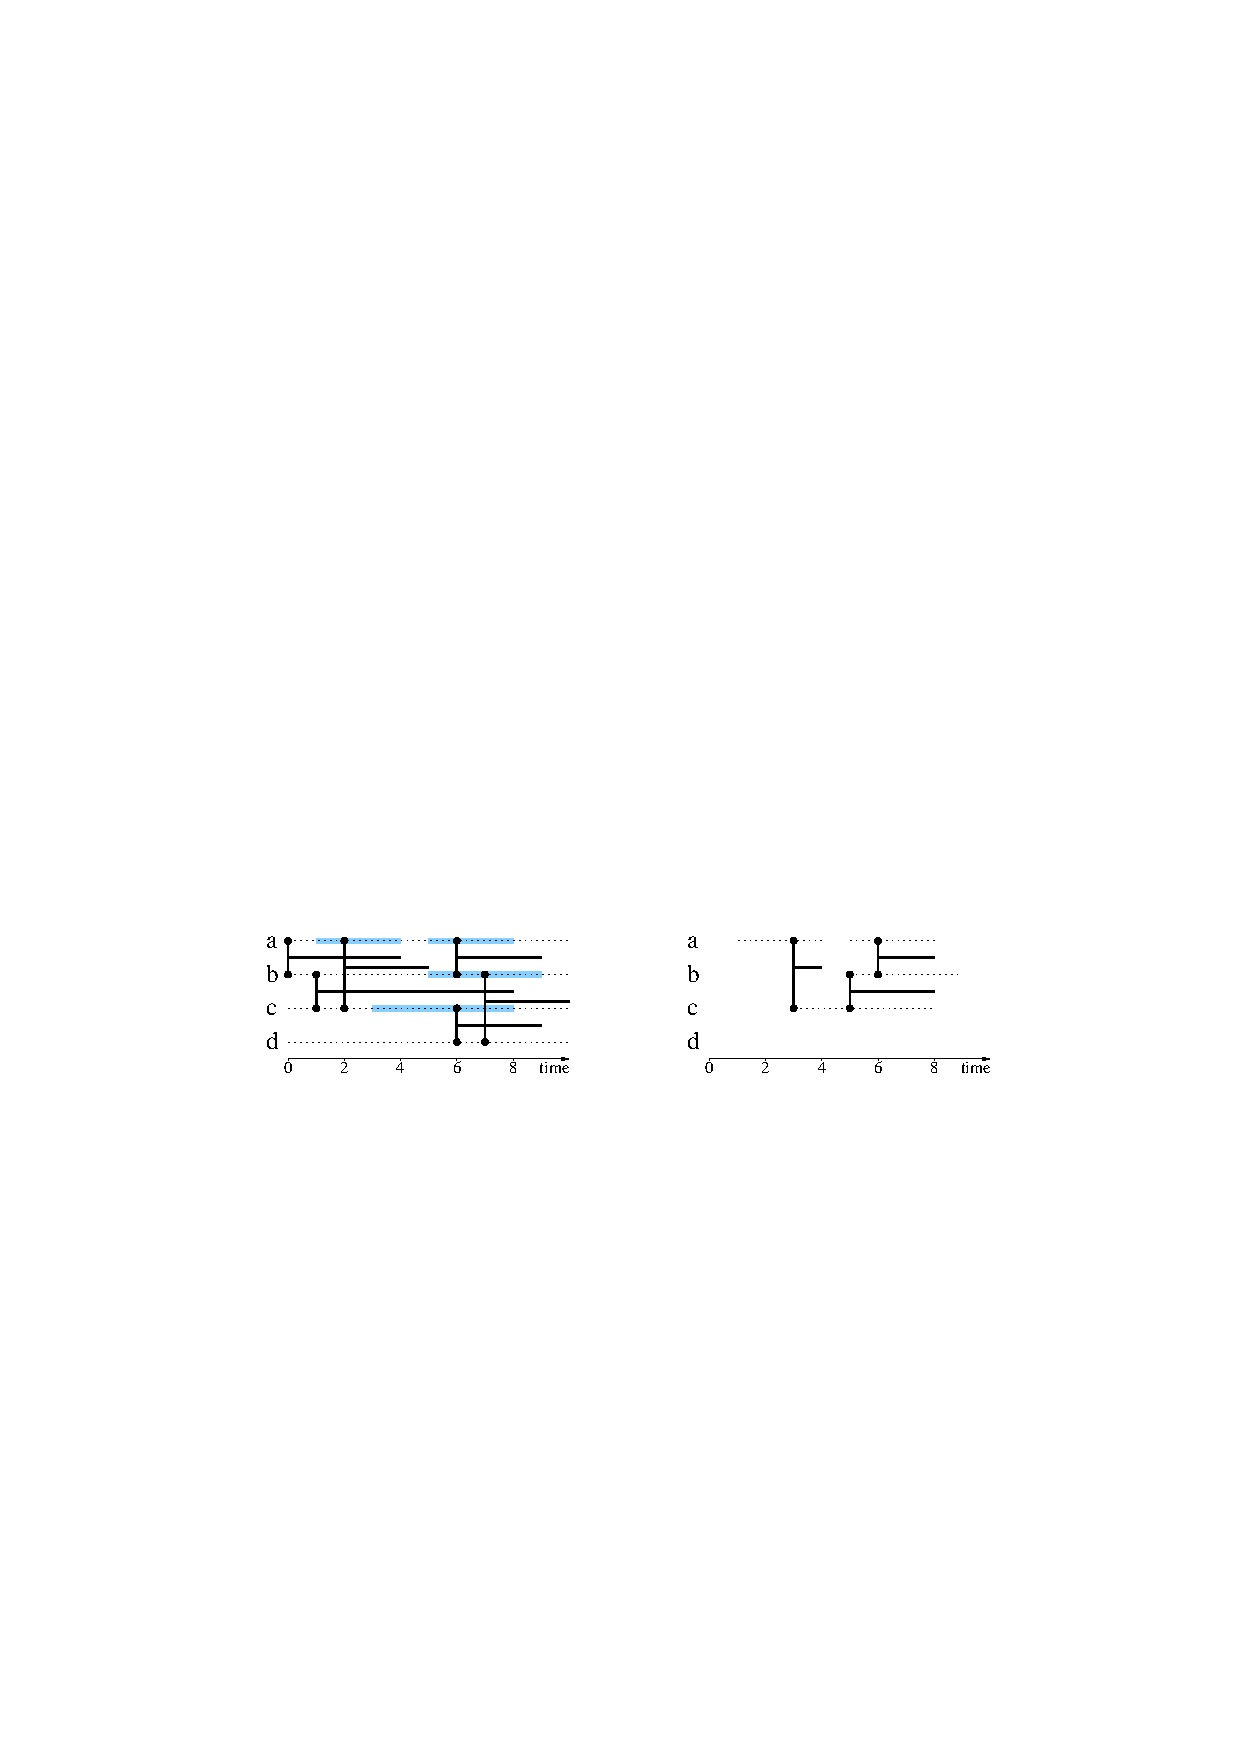
\includegraphics[width=0.9\linewidth]{pics/substream.pdf}}
\colorbox{white}{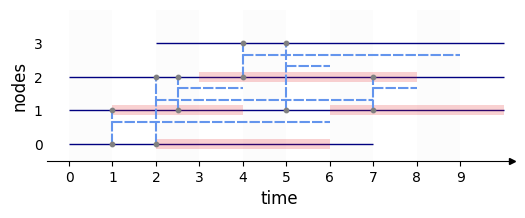
\includegraphics[width=0.45\linewidth]{pics/dynamic/cluster.png}}
\colorbox{white}{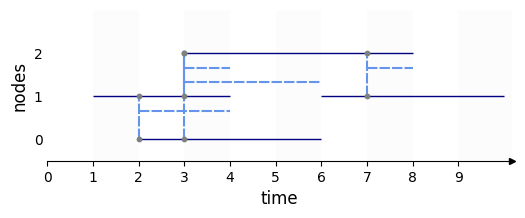
\includegraphics[width=0.45\linewidth]{pics/dynamic/subnet.png}}

Example of subgraph (red,left) and induced substream (right).

\end{textbox}







\begin{textbox}{SG - Cliques}
Having defined substreams and density, we can now naturally define a clique by analogy with static networks as a substream of density 1. A clique is said to be a \textbf{maximal clique} if it is not included in any other clique.

\centering

\vspace{0.3cm}

%\colorbox{white}{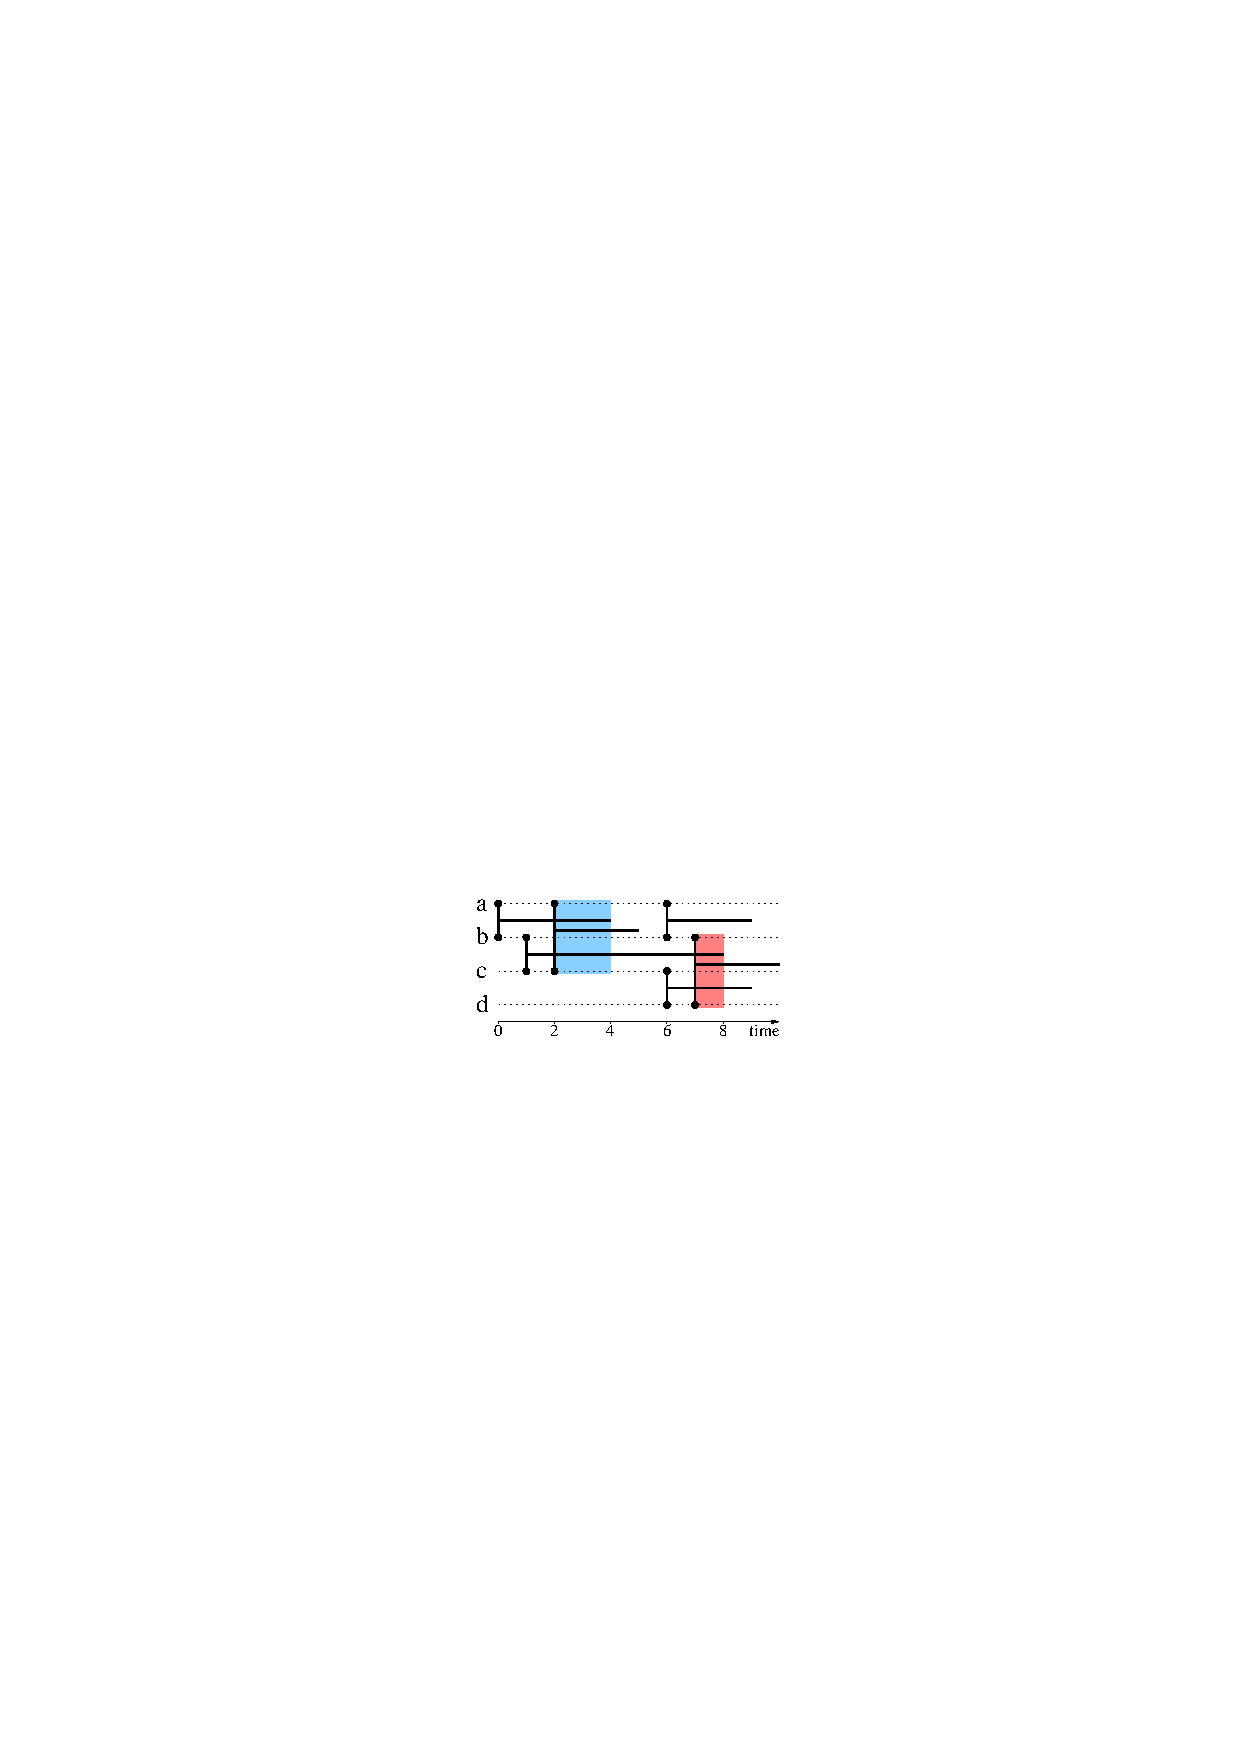
\includegraphics[width=0.8\linewidth]{pics/SGcliques.pdf}}
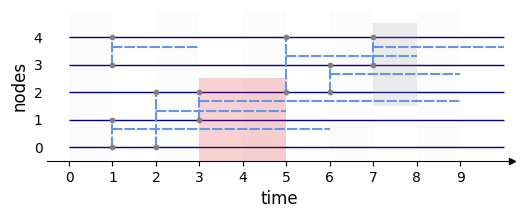
\includegraphics[width=0.9\linewidth]{pics/dynamic/cliques.png}

Red and Grey are the two maximal cliques of size three in this Stream Graph.

\end{textbox}







\begin{textbox}{SG - Neighborhood $N(u)$}
The neighborhood $N(u)$ of node $u$ is defined as the cluster composed of node-times such as an edge-time exists between it and a node-time of $u$, i.e., 
\[
N(u)= \{v_t,(u,v)_t \in E\}
\]

\end{textbox}





\begin{textbox}{SG - Degree $k(u)$}


The degree $k(u)$ of node $u$ is defined as the quantity of node in the Neighborhood of node $u$, i.e. 
\[
k(u)=|N(u)|
\]


\centering
\colorbox{white}{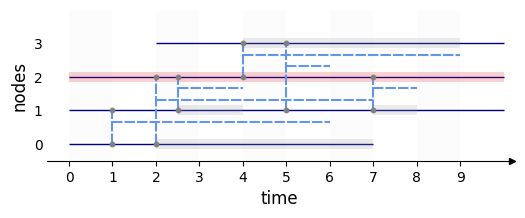
\includegraphics[width=0.7\linewidth]{pics/dynamic/neighborhood.png}}

Example, the neighborhood of node $2$ is highlighted in grey. \\$k(c)=\frac{5+2.5+5}{10}=1.25$.


\end{textbox}





\begin{textbox}{SG - Ego-network}
The Ego network $G_u$ of node $u$ is defined as the substream induced by its neighborhood, i.e., $G_u=(T,V,N(u),E(N(u)))$.


\end{textbox}





\begin{textbox}{SG - Clustering coefficient}
The clustering coefficient $C(u)$ of node $u$ is defined as the density of the ego-network of $u$, i.e., 
\[
C(u)=d(N(u))
\]

\end{textbox}





\begin{textbox}{SG - Paths}
In a Stream Graph S=(T,V,W,E), a \textbf{path} $P$ from node-time $x_\alpha$ to node-time $y_\omega$ is a sequence $(t_0,x,v_0),(t_1,v_0,v_1),...,(t_k,v_k,y)$ of elements of $T \times V \times V$ such that $t_0\geq \alpha$,$t_k\leq\omega$, $((t_i,u_i,v_i))\in E$. 

We say that $P$ \textbf{starts at} $t_0$, \textbf{arrives at} $t_k$, has \textbf{length} $k+1$ and \textbf{duration} $t_k-t_0$.

\centering
%\colorbox{white}{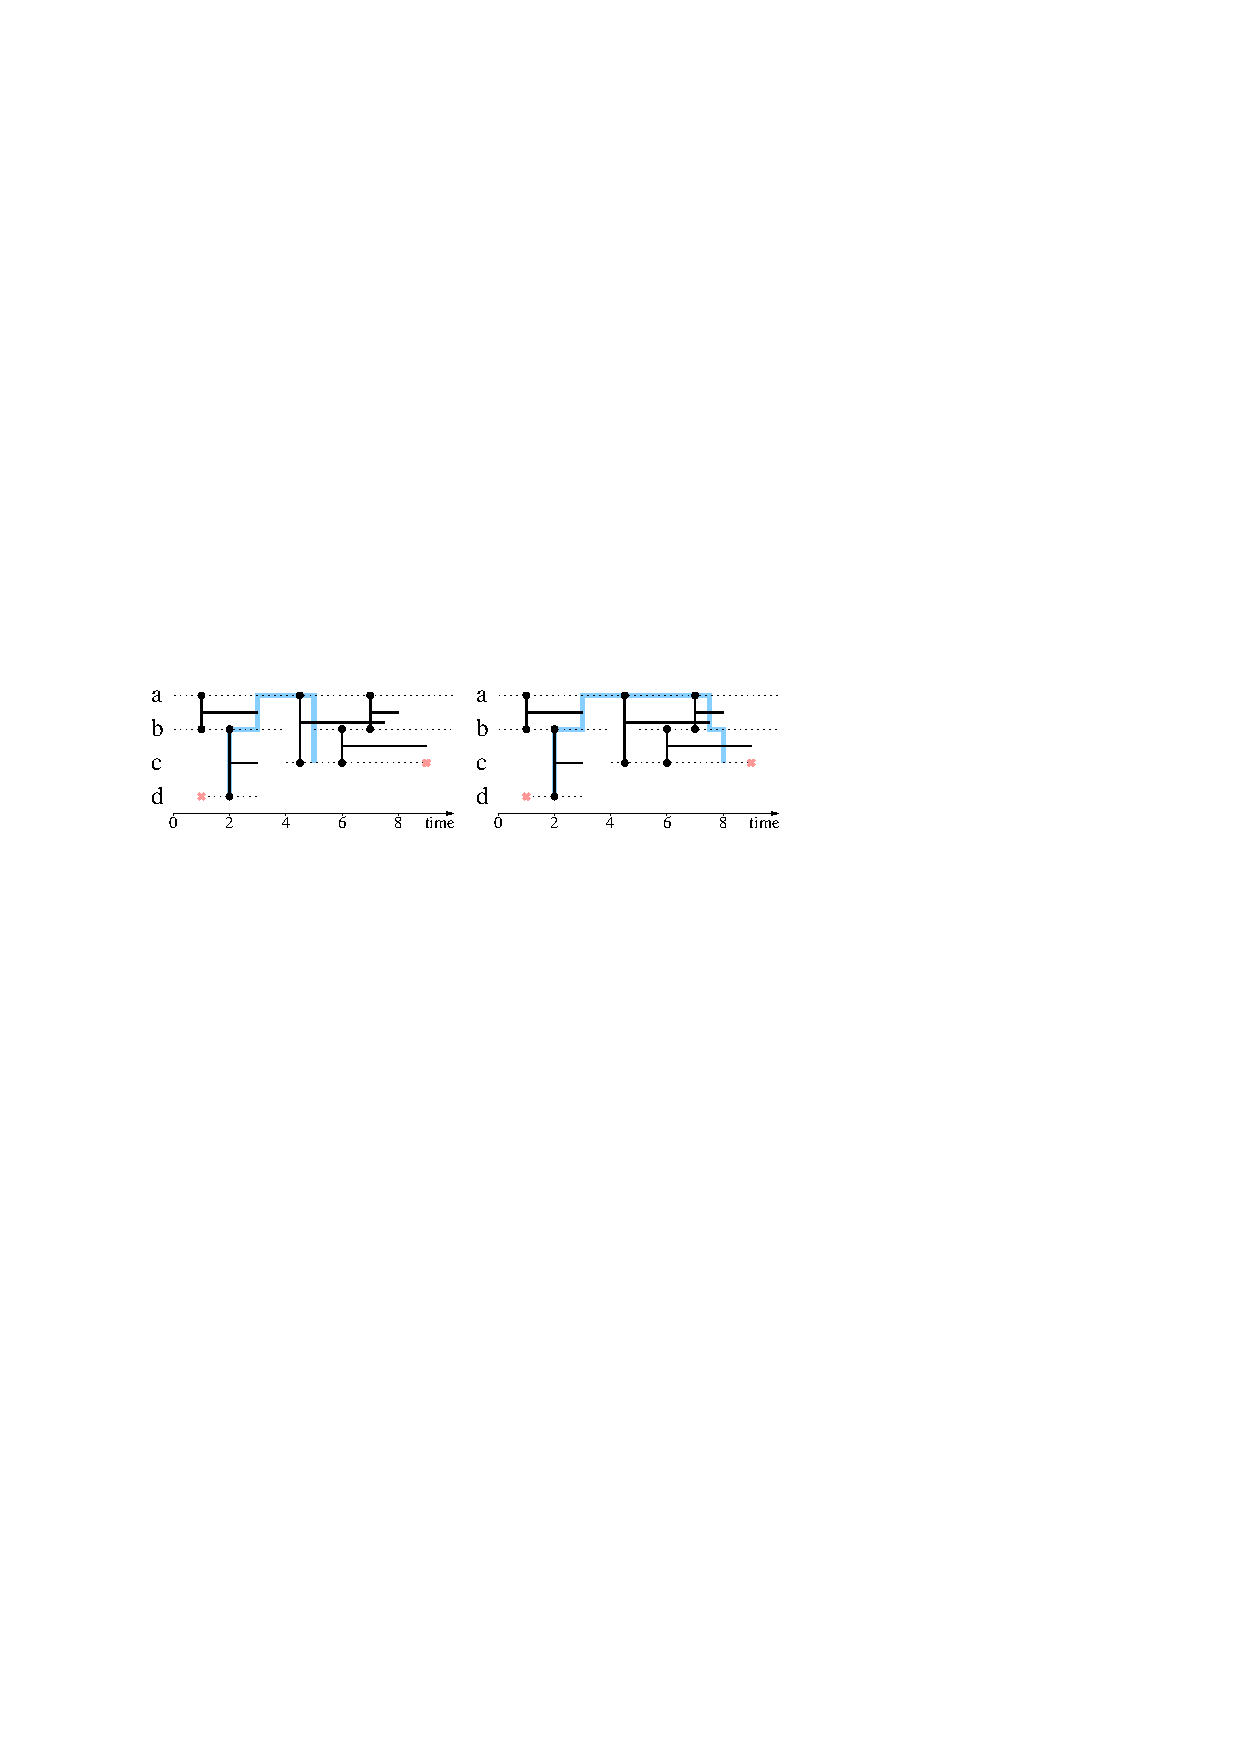
\includegraphics[width=0.8\linewidth]{pics/SGpaths.pdf}}
\colorbox{white}{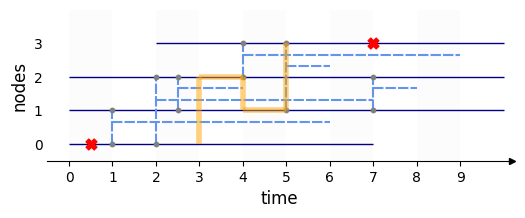
\includegraphics[width=0.45\linewidth]{pics/dynamic/path1.png}}
\colorbox{white}{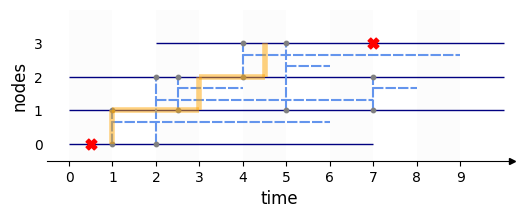
\includegraphics[width=0.45\linewidth]{pics/dynamic/path2.png}}

Examples of two paths from (node 0, t=0.5) to (node 3, t=1). The left one starts at 3, arrives at 5, has length 3 and duration 2. The right one starts at 1, arrives at 4.5, has length 3 and duration 3.5.
\end{textbox}


\begin{textbox}{SG - Shortest - Fastest - Foremost}
\begin{itemize}
    \item \textbf{Shortest Paths}, as in static networks, are paths of \textbf{minimal length}.
    \item \textbf{Fastest Paths} are paths of \textbf{minimal duration}.
    \item \textbf{Foremost Paths} are paths \textbf{arriving first}.
\end{itemize}

Furthermore, one can combine those properties, defining for instance:

\textbf{Fastest shortest paths} (paths of minimum duration among those of minimal length)

\textbf{Shortest fastest paths} (paths of minimal length among those of minimal duration)

\end{textbox}

\begin{textbox}{SG - Shortest - Fastest - Foremost}
\centering
\colorbox{white}{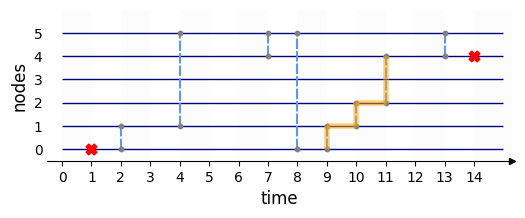
\includegraphics[width=0.45\linewidth]{pics/dynamic/fastest.png}}
\colorbox{white}{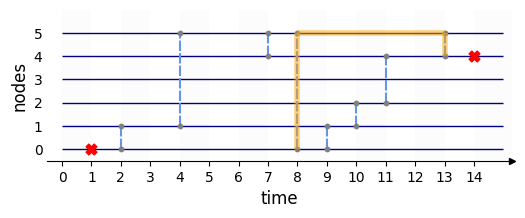
\includegraphics[width=0.45\linewidth]{pics/dynamic/shortest.png}}
\colorbox{white}{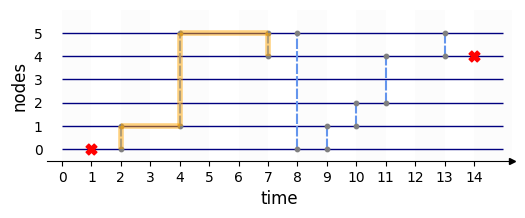
\includegraphics[width=0.45\linewidth]{pics/dynamic/foremost.png}}

Fastest (top left),  Shortest (top right), Foremost (bottom),

\end{textbox}

\begin{textbox}{SG - Connected Components}

Various definitions for connected components have been proposed for temporal networks, see  (\cite{latapy2018stream}) for details. One of the simplest one is the \textbf{weakly connected component}, defined such as two node-times belong to the same connected component if and only if there is a path from one to the other, \textit{ignoring time}. 

\centering
%\colorbox{white}{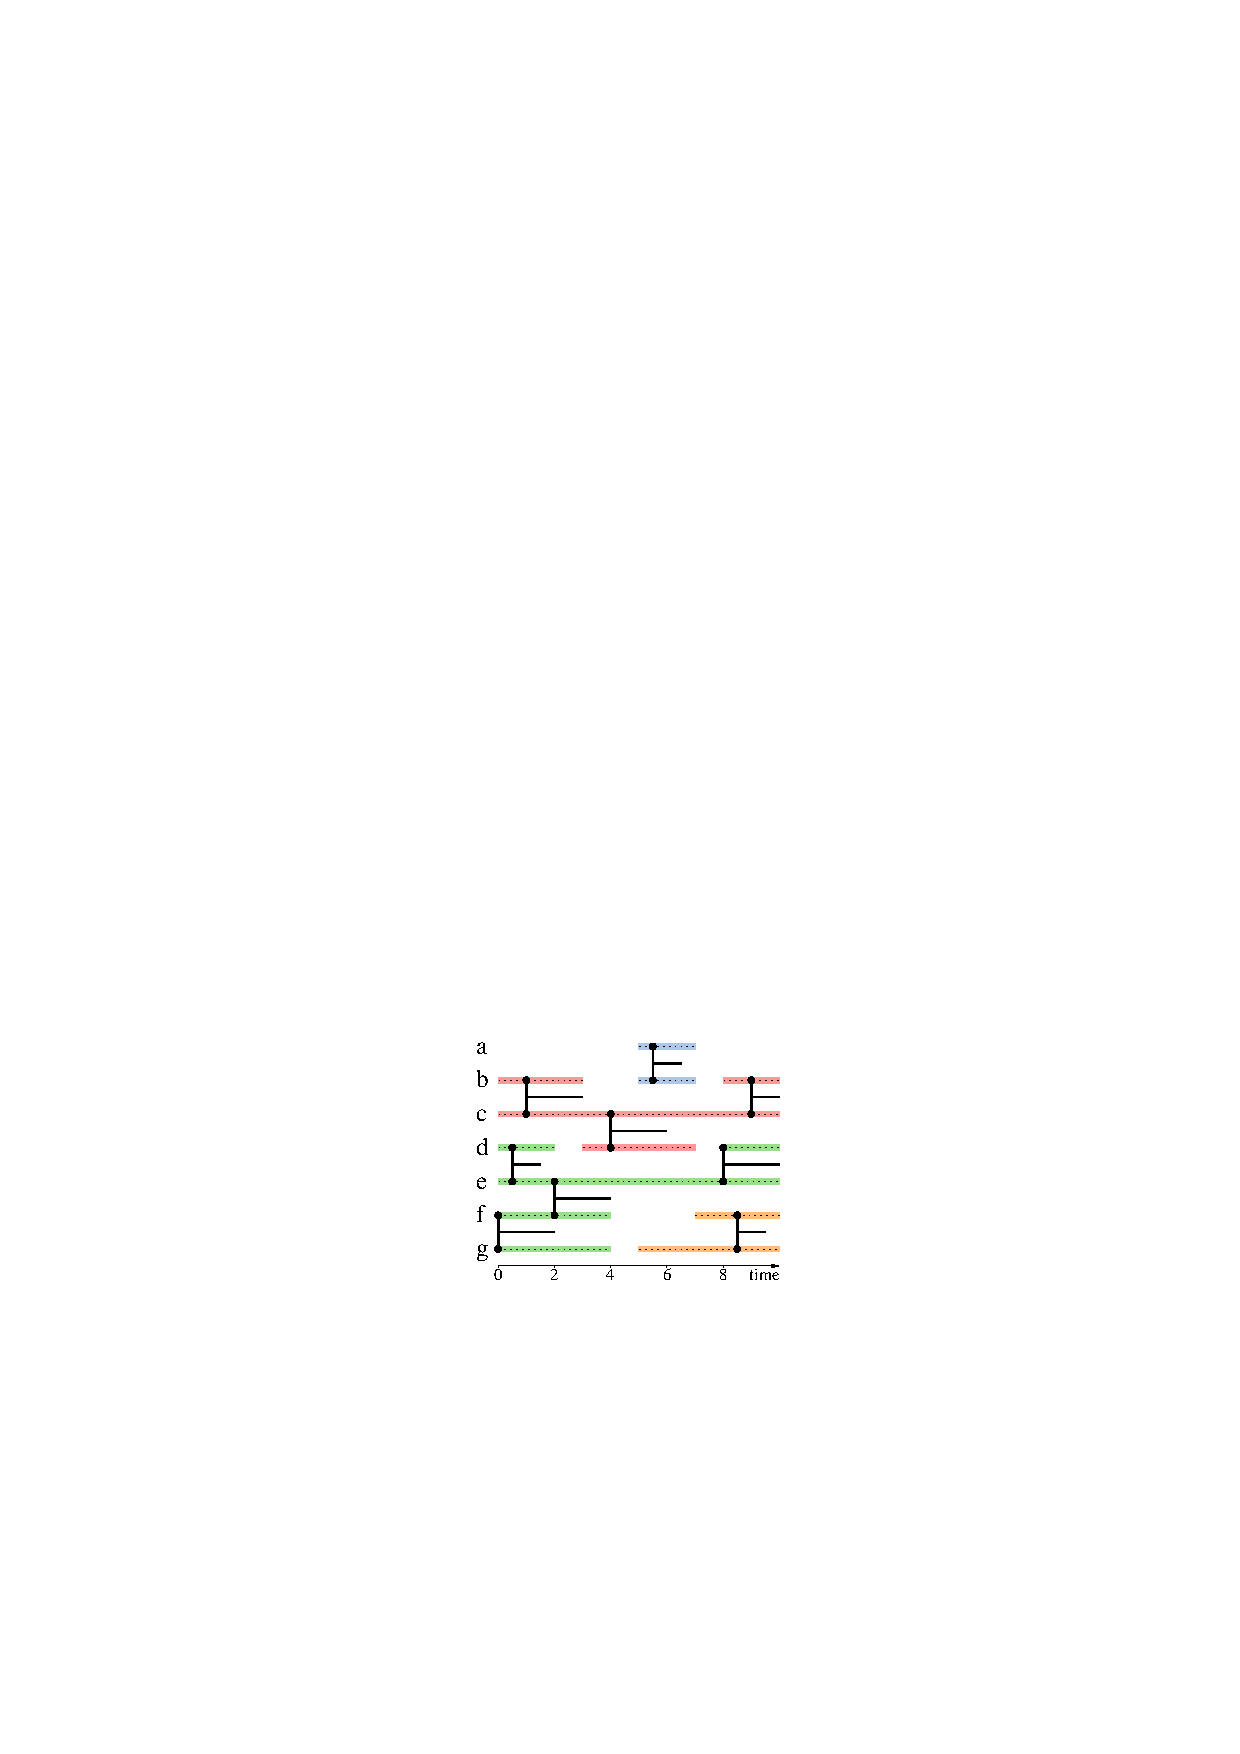
\includegraphics[width=0.6\linewidth]{pics/SGweakCC.pdf}}
\colorbox{white}{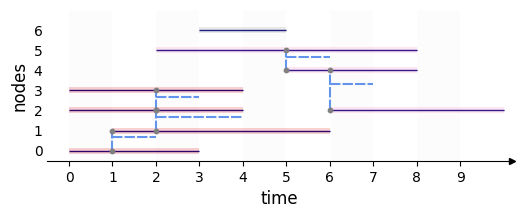
\includegraphics[width=0.8\linewidth]{pics/dynamic/CC.png}}

Example of a Stream Graph decomposed in 3 weakly connected components (including one composed of the singleton node 6)
\end{textbox}






\begin{textbox}{Random Models}

We have seen that comparing an observed network with a randomized version of it has many applications. In dynamic networks, many variants have been proposed. In (\cite{gauvin2018randomized}), the authors consider methods defined on sequences of snapshots that conserve nodes and number of events, and grouped them in 4 main families, \textbf{Snapshot Shuffling, Sequence Shuffling, Link Shuffling} and \textbf{Timeline Shuffling}.

\end{textbox}




\begin{textbox}{Snapshot Shuffling}

 \textbf{Snapshot Shuffling} keeps the order of snapshots, randomize edges inside snapshots. Any random model for static network can be used, such as ER random graphs or a degree preserving randomization.
 
 
 
\centering
\colorbox{white}{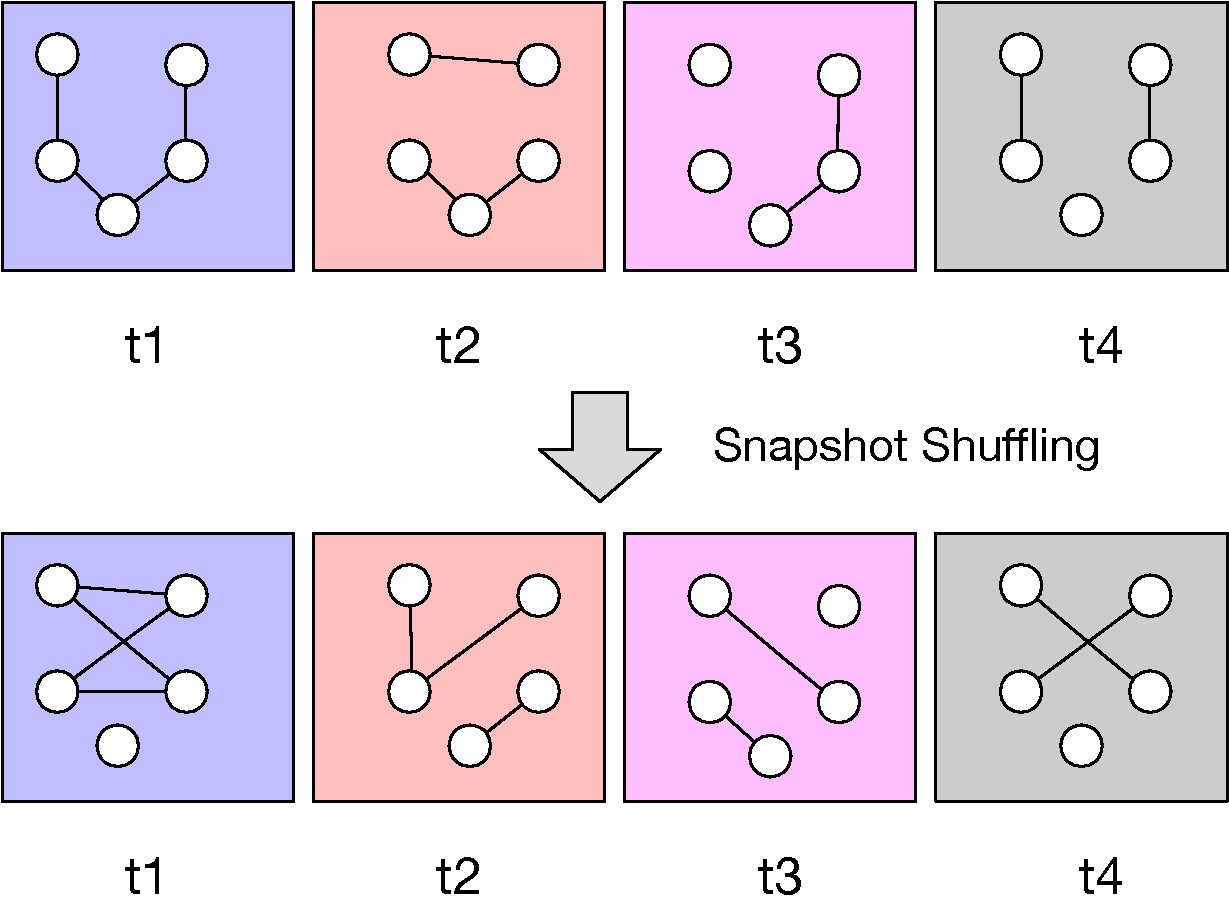
\includegraphics[width=0.8\linewidth]{pics/dynamic/snapshot_shuffling.pdf}}
 
\end{textbox}



\begin{textbox}{Sequence Shuffling}
 \textbf{Sequence Shuffling} keeps each snapshot identical, switch randomly their order. 
 
 
 
\centering
\colorbox{white}{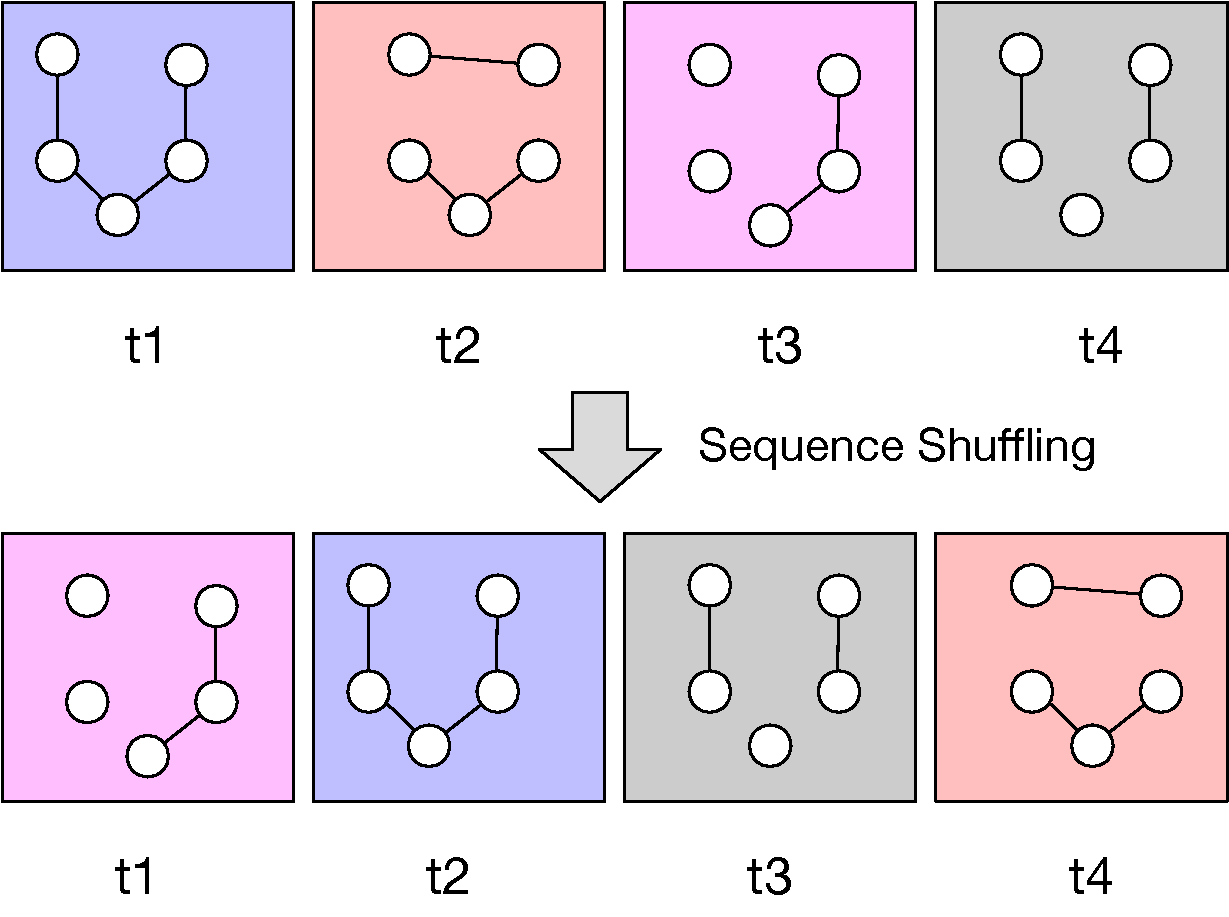
\includegraphics[width=0.8\linewidth]{pics/dynamic/squence_shuffling.pdf}}
 
\end{textbox}





\begin{textbox}{Link Shuffling}
 \textbf{Link Shuffling} keeps activation time per node pairs, randomize the aggregated graph. For instance, a simple way to achieve this is to pick two node pairs at random (connected or not) of the aggregated graph, and to exchange activation time of these node pairs, e.g.:
   
%   \[
%   (u_1,u_2):{t_1,t_2,...},(u_3,u_4):{t_3,t_4,...} \xrightarrow{}(u_1,u_2):{t_3,t_4,...},(u_3,u_4):{t_1,t_2,...}
%   \]

 
 
\centering
\colorbox{white}{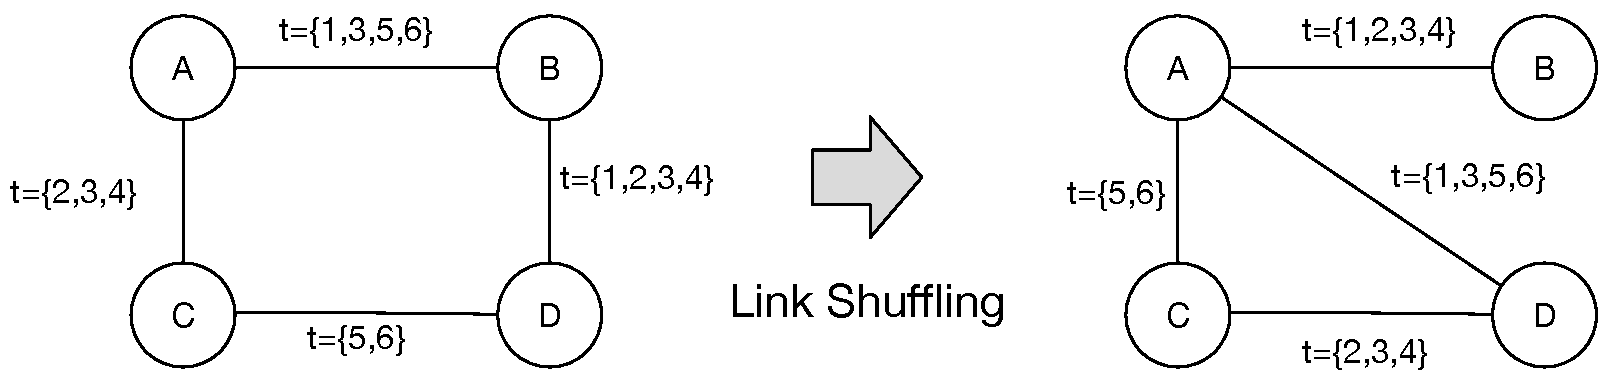
\includegraphics[width=0.9\linewidth]{pics/dynamic/link-shuffling.pdf}}
 
\end{textbox}



\begin{textbox}{Timeline Shuffling}
\textbf{Timeline Shuffling} keeps the aggregated graph, randomize edges activation time. For instance, a simple way to achieve this is to redistribute randomly activation period among all edges, e.g.: 
   
%  \[
%  (u_1,u_2,t_1),(u_2,u_3,t_2) \xrightarrow{}(u_1,u_2,t_2),(u_2,u_3,t_1)
%  \]
% Unlike in Link shuffling, the number of observations of each edge is conserved.
 
 
\centering

\colorbox{white}{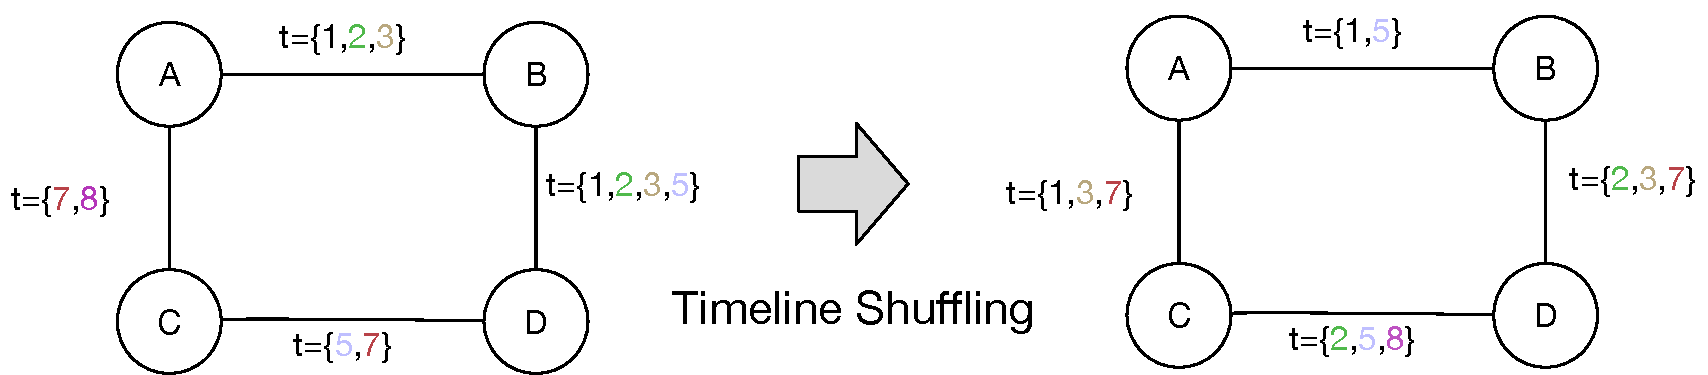
\includegraphics[width=0.9\linewidth]{pics/dynamic/timeline-shuffling.pdf}}
 
\end{textbox}

\begin{textbox}{More constrained Shuffling}
Variants of these shufflings with additional constraints have been proposed, for instance the \textbf{Local timeline shuffling}, randomizing events time edge by edge, or the \textbf{Weight constrained timeline shuffling}, randomizing events while conserving the number of observations for each edge. See (\cite{gauvin2018randomized}) for more.
 
 
\centering

%\colorbox{white}{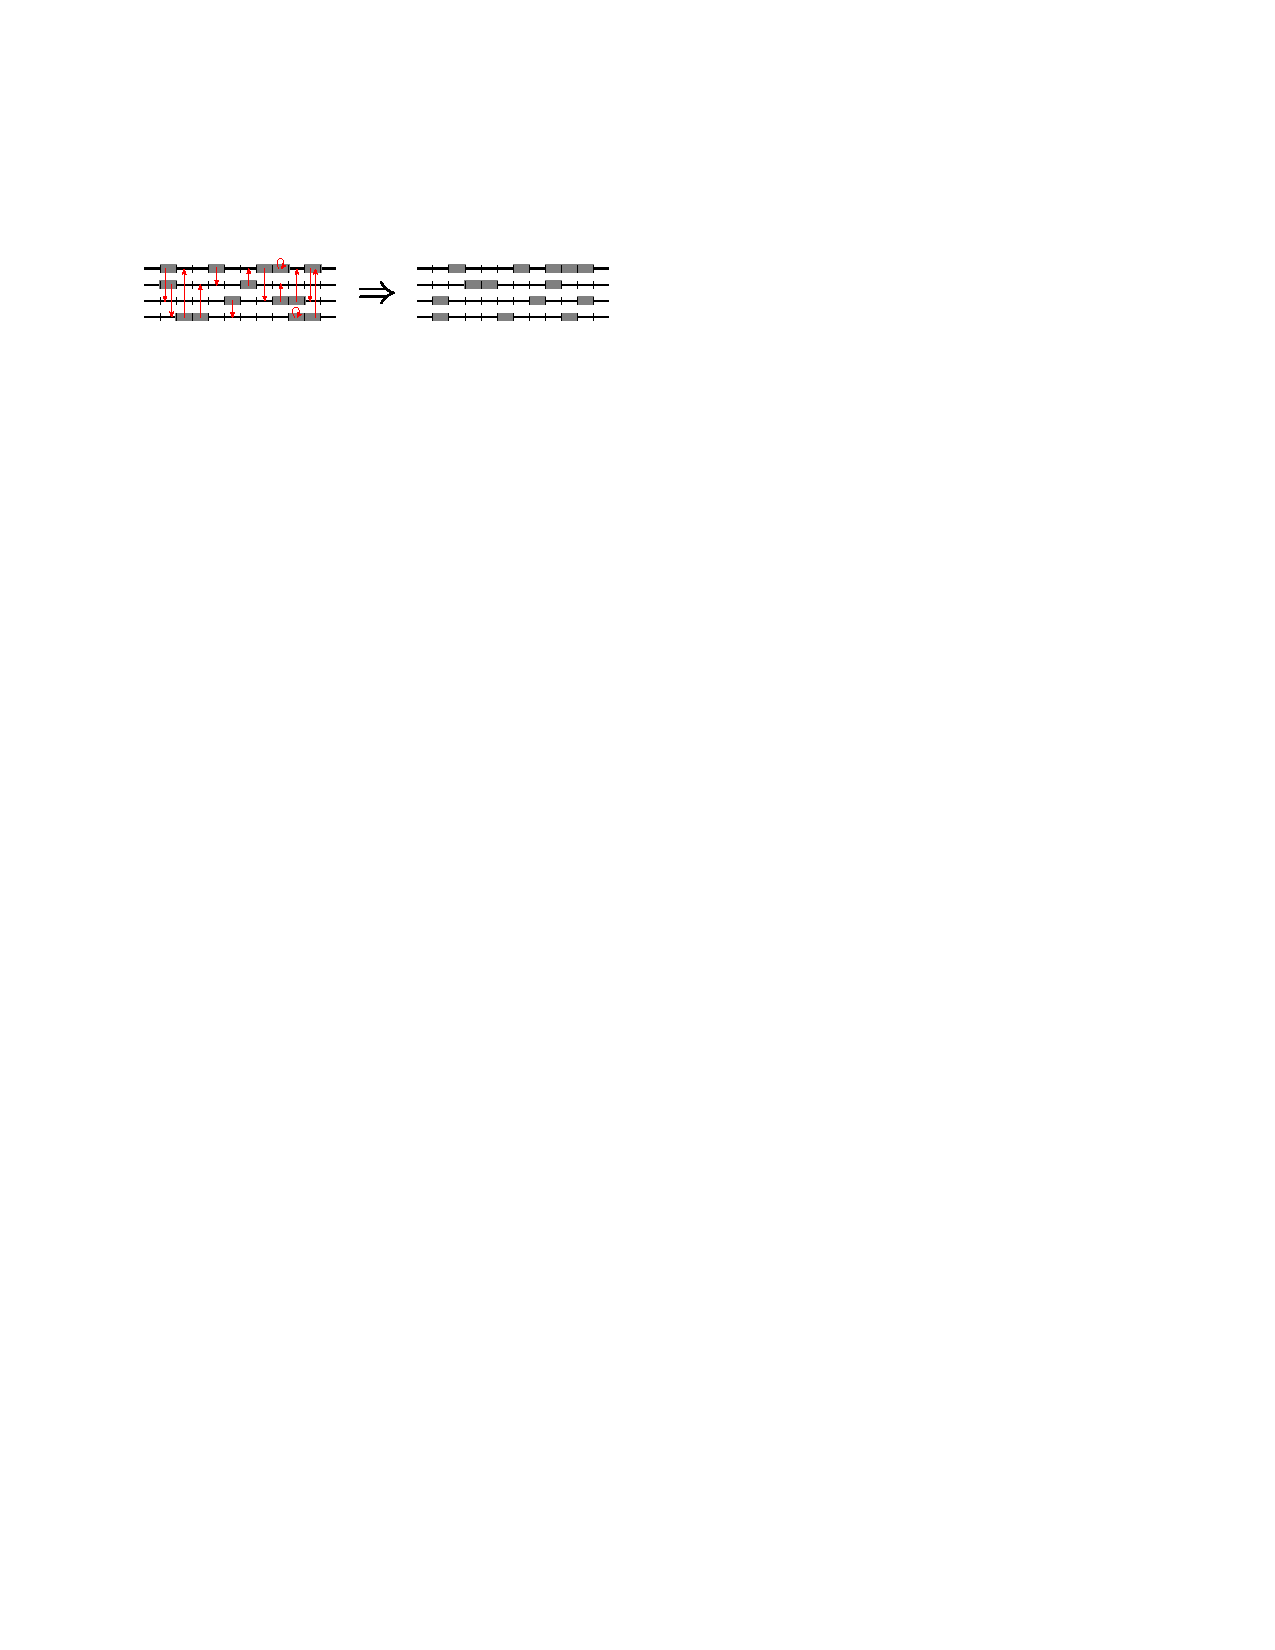
\includegraphics[width=0.7\linewidth]{pics/timelinesuffling2.pdf}}
 
\end{textbox}


\begin{textbox}{Going Further}
Book: \cite{holme2019temporal}

Stream Graph definition: \cite{latapy2018stream}

Transforming dynamic networks into static networks:  \cite{kivela2018mapping}

Dynamic Communities: \cite{rossetti2018community}

\end{textbox}
 \AtNextBibliography{\footnotesize}


\printbibliography[heading=subbibliography]


\end{multicols}



\end{document}


